
\documentclass[conference]{IEEEtran}


\usepackage{graphicx}
\usepackage{float}




\hyphenation{op-tical net-works semi-conduc-tor}
\usepackage{amsmath}


\begin{document}
%
% paper title
% can use linebreaks \\ within to get better formatting as desired
\title{Near Real-Time Vehicle Detection and Tracking in Highways}


% author names and affiliations
% use a multiple column layout for up to three different
% affiliations
\author{\IEEEauthorblockN{Ebrahim Soroush}
\IEEEauthorblockA{Amirkabir University of Technology\\ Email: e.soroush@hotmail.com}
\and
\IEEEauthorblockN{Ali Mirzaei}
\IEEEauthorblockA{Amirkabir University of Technology\\
Email: a.mirzaei69@gmail.com}
\and
\IEEEauthorblockN{Shiva Kamkar}
\IEEEauthorblockA{Amirkabir University of Technology\\
Email: shv.kamkar@gmail.com}}

\bibliographystyle{IEEEtran}

% make the title area
\maketitle


\begin{abstract}
%\boldmath
In this paper we present an approach for detection and tracking of vehicles in highways. The Aggregated Channel Features (ACF) are used to detect vehicles and the Kalman filter is employed to track the detected objects. The proposed scheme enjoys high accuracy in both detection and tracking. Moreover, it can be run at near real-time speed on an ordinary computer (both detection and tracking take about 140ms for each frame). The proposed approach was the best algorithm in AUTCUP2015 competitions and it got the second rank in that competition (The first rank was not given to any team).
\end{abstract}

% IEEEtran.cls defaults to using nonbold math in the Abstract.
% This preserves the distinction between vectors and scalars. However,
% if the conference you are submitting to favors bold math in the abstract,
% then you can use LaTeX's standard command \boldmath at the very start
% of the abstract to achieve this. Many IEEE journals/conferences frown on
% math in the abstract anyway.

% no keywords




% For peer review papers, you can put extra information on the cover
% page as needed:
% \ifCLASSOPTIONpeerreview
% \begin{center} \bfseries EDICS Category: 3-BBND \end{center}
% \fi
%
% For peerreview papers, this IEEEtran command inserts a page break and
% creates the second title. It will be ignored for other modes.
\begin{IEEEkeywords}
	Detection, Tracking, ACF, Kalman Filter, Vehicle
\end{IEEEkeywords}

\section{Introduction}

With daily increasing of number of vehicles and highway traffics, the Intelligent Traffic Systems (ITS) become more and more important than before. Obtaining the traffic parameters such as number of vehicles, average speed for any type of vehicles (light and heavy) and etc. can help the responsible organizations with better monitoring of the traffic. The vision-based systems are better than other existing methods (like laser guns for obtaining the speed or magnetic loops for counting and classification of vehicles) from several point of view: first, the cost of these kind of systems are far less than others. Secondly, the maintenance of cameras are much easier and thirdly all traffic parameters can be obtain with a single camera in a specific area. 


In this paper we propose a scheme to detect and track vehicles in a video. Our proposed scheme works on a single camera which mounted on a high place and it is recording video from rear of vehicles. Moreover, it can be used in other views of camera if the detection model is trained based on that given view. The Aggregated Channel Features (ACF) is used for detection and a Kalman filter is employed to track the vehicles. The proposed approach can detect and track the vehicles in a near real-time speed (about 5 frame per second) on an ordinary computer\footnote{Intel i5-4460, 8GB RAM}. The presented approach was the best method in AUTCUP2015 competitions in Amirkabir University of Technology and it ranked second in that competitions (no team ranked first).



The rest of this paper is organized as follow: Section II illustrates the existing algorithms. In section III the used detection algorithms (ACF) is described. In section IV the configuration of out kalman filter as a tracker is explained and section V concludes the paper. 
\section{Related Works}
Detection and tracking of vehicles can be considered as a core of a vision-based intelligent system. In the following subsections the most well-known methods for both detection and tracking are reviewed and the reasons of selected methods are presented.
\subsection{Detection}



\begin{figure*}
	\centering
	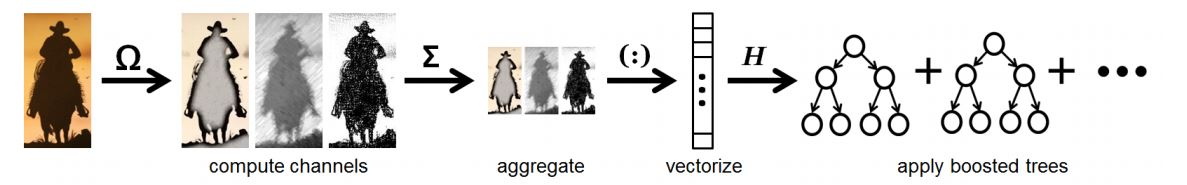
\includegraphics[width=\textwidth]{images/acfSteps.JPG}
	\caption{Outline of Aggregated Channel Features framework. First step: Computing several channels of given image $I$ with $\Omega$. Second step: Sum every blocks of channel features and smooth the resulting aggregated channels. Third step: Concatenation of feature channels in a vector. Fourth step: Training a boosted classifier \cite{dollar2014fast}}
	\label{ACFSteps}
\end{figure*}



All detection algorithms can be classified into two categories: motion-based and appearance-based approaches. Motion-based methods \cite{sen2004robust},\cite{sirikuntamat2015vehicle},\cite{lu2014moving} try to detect vehicles using their motions. However, these methods are fast and easy (they do not need to be trained), they are so vulnerable to shadows, luminance changes and shaking of the camera. In the other hand appearance-based approaches detect vehicles with a pre-trained model according to the intrinsic features of objects. Generally these kind of methods are more  computationally demanding than motion-based approaches but they do not have the mentioned disadvantages of these methods.

As mentioned the appearance-based detections are more robust against luminance changed, camera shaking and shadows (problems that are common on highways). Because of these reasons we chose this family of methods for detection task. 

One of the most well-known methods in object detection are part-based models such Deformable Part Model (DPM) \cite{felzenszwalb2008discriminatively}. Although DPM has a convincing performance for vehicle detection, it suffers from a high computations in test phase. The time consumption of DPM in test phase prevent us to have a real-time or even near real-time system for detection and tracking of vehicles. There are some methods which try to get fast DPM \cite{} but all these algorithms reduce the performance or they are not real-time.

Recently the Convolutional Neural Networks (CNNs) presented very good results in object detection. These kind of methods are state-of-the-art algorithm in object detection.


\subsection{Tracking}
Generally there are two approaches to track objects. First, tracking by detection, in which objects are detected in each frame and they are linked up in consecutive frames. Secondly, tracking by matching, that they tracked a predefined object in the next frames.


\section{Detection}
This section provides a brief overview of ACF detection \cite{dollar2014fast} method. This method has a high accuracy for object detection tasks (especially solid objects) comparing with other competing algorithms \cite{dollar2010fastest}. Moreover, it enjoys a very high speed in both training and test stages. In the subsequent sections, feature types of this method are introduced and also it is explained how to extract these features in a fast way.

\subsection{Aggregated Channel Features (ACF)}
The ACF method could be summarized into four major steps.
First step includes computing several channels for a given image $I$ with a transformation function $C=\Omega({I})$. In the second step, each channel features is partitioned to some blocks and summation in every block leads to a lower resolution channel. Finally the aggregated features will be obtained with applying a smoothing filter on the lower resolution channels. Next step is concatenating of all pixels in the aggregated channels in a vector. In the last step, a boosted trees of classifier is trained to distinguish objects from background. Fig \ref{ACFSteps} demonstrates these steps. 

The main features of ACF detector can be summarized as:

\textbf{Channels:} 
 10 channels of features are extracted as: LUV color channels (3 channels), normalized gradient magnitude (1 channel) and histogram of oriented gradients (6 channels). After smoothing these channels with a 
$[1\ 2\ 1]/4$ filter, 
the channels divided into $4 \times 4$ blocks and pixels in each block are summed up. Finally the channels are smoothed again with the same filter.

\textbf{Classifier:} For classifying of cars and non-cars, an AdaBoost classifier \cite{friedman2000additive} is trained which uses 128 depth-two trees as weak classifiers.

\textbf{Sliding Window Detection:} As traditional object detectors, sliding window scheme is employed to find the bounding boxes of car candidates. In this approach extracted features in multiple scales, called feature pyramid, fed into a boosted classifier. Calculating of this feature pyramid usually is a bottleneck of the running time of detection. In the next section this subject will be covered in detail.

\subsection{Fast Feature Pyramids}
One of the most challenging problems in object detection is that different instances of one object could be appeared in different sizes. To tackle this problem, detectors use sliding window method in a pyramid of multiple scale images. In traditional methods it was needed to calculate features in every scales. Therefore, constructing the feature pyramid  resolves the multi-scale problem by increasing the computational cost.

 To accelerate feature pyramid extraction, the ACF detector approximates features in different scales instead of calculating them. For clarifying the subject, let $I_{k}(x,y)=I(x/k,y/k)$ is the up-sampled version of original image and desired features are gradient of the image. Following the simple derivative rules:
  $$h_{k_x} = \frac{\partial I_k}{\partial x}(x,y)=\frac{1}{k}\frac{\partial I}{\partial x}(x/k,y/k)$$ $$h_{k_y} = \frac{\partial I_k}{\partial y}(x,y)=\frac{1}{k}\frac{\partial I}{\partial y}(x/k,y/k)$$ With a simple calculus we can deduce that $h_k=k\times h$.
  
Besides above formulas, experiments also show approximation $h_{k}\approx k\times h$ for gradient histogram features is true.  Because of information lost in down-sampled images, these formulas are no longer valid. But experiments show this information lost is consistent and could be approximated with $h_{1/k}\approx \mu h$, where $\mu$ is a constant value smaller than $1/k$.
More details and result of experiments are presented in \cite{dollar2014fast}.
\begin{table*}[t] \label{tableResult}
	\caption{Comparison of our results with other teams in AUTCUP competition}
	\centering
	\begin{tabular}{c||ccccccccccc}
		\hline
		Team&Recall&Precision&FAR&MT&ML&FP&FN&IDs&FM&MOTA&MOTP\\
		\hline
		\textbf{AVId}&\textbf{51.27}&\textbf{81.49}&2.93&\textbf{97}&\textbf{133}&17961&\textbf{75144}&\textbf{91}&\textbf{380}&\textbf{39.57}&\textbf{73.54}\\
		FanAsaa&43.45&64.59&6.01&95&157&36737&87210&667&1072&19.20&73.49\\
		Basir&12.95&54.56&\textbf{2.72}&27&383&\textbf{16632}&134260&127&426&2.08&68.3\\
		\hline
	\end{tabular}
	
\end{table*}


\section{Tracking: Kalman Filter}
We use the Kalman filter framework for tracking of a single object. In first subsection the model specification of this Kalman filter is explained and in the second part we introduce  an assignment algorithm  to extend the single object tracking to a multi-object one.
\subsection{Kalman Model}
We consider position ($x,y$) and size of bounding box ($w,h$) and their velocity as the state of Kalman filter. So the state of the kalman filter will have 8 variables ($x,y,w,h,v_x,v_y,v_w,v_h$).
With this defining of these variables the dynamic model will be:

\[
\begin{bmatrix}
x \\
y \\
w \\
h \\
v_x \\
v_y \\
v_w \\
v_h
\end{bmatrix}^{t+1}
=
\begin{bmatrix}
1 &0 & 0 & 0  & 1 & 0 &0 &0 \\
0 &1 & 0 & 0  & 0 & 1 &0 &0 \\
0 &0 & 1 & 0  & 0 & 0 &1 &0 \\
0 &0 & 0 & 1  & 0 & 0 &0 &1 \\
0 &0 & 0 & 0  & 1 & 0 &0 &0 \\
0 &0 & 0 & 0  & 0 & 1 &0 &0 \\
0 &0 & 0 & 0  & 0 & 0 &1 &0 \\
0 &0 & 0 & 0  & 0 & 0 &0 &1 \\
\end{bmatrix}
\begin{bmatrix}
x \\
y \\
w \\
h \\
v_x \\
v_y \\
v_w \\
v_h
\end{bmatrix}^t+n_d,
\]

where $n_d$ is a vector and called model noise. The measurement model can be written as following:

\[
\begin{bmatrix}
x \\
y \\
w \\
h \\
\end{bmatrix}
=
\begin{bmatrix}
1 &0 & 0 & 0  & 0 & 0 &0 &0 \\
0 &1 & 0 & 0  & 0 & 0 &0 &0 \\
0 &0 & 1 & 0  & 0 & 0 &0 &0 \\
0 &0 & 0 & 1  & 0 & 0 &0 &0 \\

\end{bmatrix}
\begin{bmatrix}
x \\
y \\
w \\
h \\
v_x \\
v_y \\
v_w \\
v_h
\end{bmatrix}+n_m
\],

where $n_m$ is a vector and is called the measurement noise. 


\subsection{Assignment of Detections and Tracks}

The following cost matrix is used to assign the detected objects to existing tracks:
\begin{equation}\nonumber
c(i,j)= \frac{Area(d_i\cap t_j)}{\sqrt{Area(d_i)*Area(t_j)}},
\end{equation}

where $d_i$ and $t_j$ are the bounding box of $i^{th}$ detection and $j^{th}$ track, respectively. The Hungarian algorithm \cite{} is used to assign the detections and tracks according to defined cost matrix. There are three types of assignments:
\begin{itemize}
\item \textbf{Assigned Pairs}\\
In this case the Kalman filter of the assigned track would be corrected with its assigned detection.

\item \textbf{Unassigned Detections}\\
An unassigned detection is probably a new object which is appeared in the current frame. So a new track will be initiated. At first the created track is not a valid track. If the number of assignment gets greater than a threshold, the track will be valid. This validation procedure help the tracker to remove the noisy false alarms of detection.

\item \textbf{Unassigned Tracks}\\	
In this case the counter of unassigned tracks will be incremented. If this counter for a particular track gets greater than a predefined threshold, that track will be killed. 
	
\end{itemize}






\section{Implementation and Performance Evaluation}
In this section we demonstrate the performance of our method on AUTCUP dataset\footnote{Available in November 2015 at: http://ceit.aut.ac.ir/~nikabadi/AAIC\_traffic\_dataset/} and explain some implementation details.\\
\subsection{Implementation}
We train ACF detector with open-source piotr-toolbox \cite{PMT}.  For convenience we used a pre-trained DPM model on PASCAL VOC2012 on the train videos for extracting car patches. In training we extract 1657 patches of cars and 19188 non-car patches all resized in $[64\ 64]$ from training videos. Training phase including reading all images, extracting feature pyramids with aforementioned method and training boosted classifiers takes 17 seconds.
AUTCUP dataset includes $12$ video of non-stable cameras from different views, Fig \ref{results} shows some samples of these videos. For training we randomly captured 1000  frames from each video and extracted car and non-car patches from these frames.

\subsection{Results} 
Table \ref{tableResult} shows result of first 3 teams of AUTCUP2015. As shown the proposed approach outperforms other participating teams in most metrics of this competitions. Particularly, our method gets MOTA of 39.57 which is almost twice better than the second team. More details of detection and tracking metrics can be found at \cite{}.
Moreover, the proposed algorithm works in near real-time (5 frame per second) on a $960\times 540$ video on a ordinary PC.
The output of tracking on all 12 videos are shown in Fig \ref{results}. 


\section{Conclusion}
In this paper we presented a feasible paradigm for detection and tracking of vehicles in highways. This method enjoys high accuracy and near real-time speed property on an ordinary PC. In more details, the running time of our algorithm in test phase is about 145 ms for each frame and it got MOTA of 39.57 and MOTP of 73.54 in AUTCUP dataset. These obtained accuracies is the best results in AUTCUP2015.

\begin{figure*}[t]
	\centering
	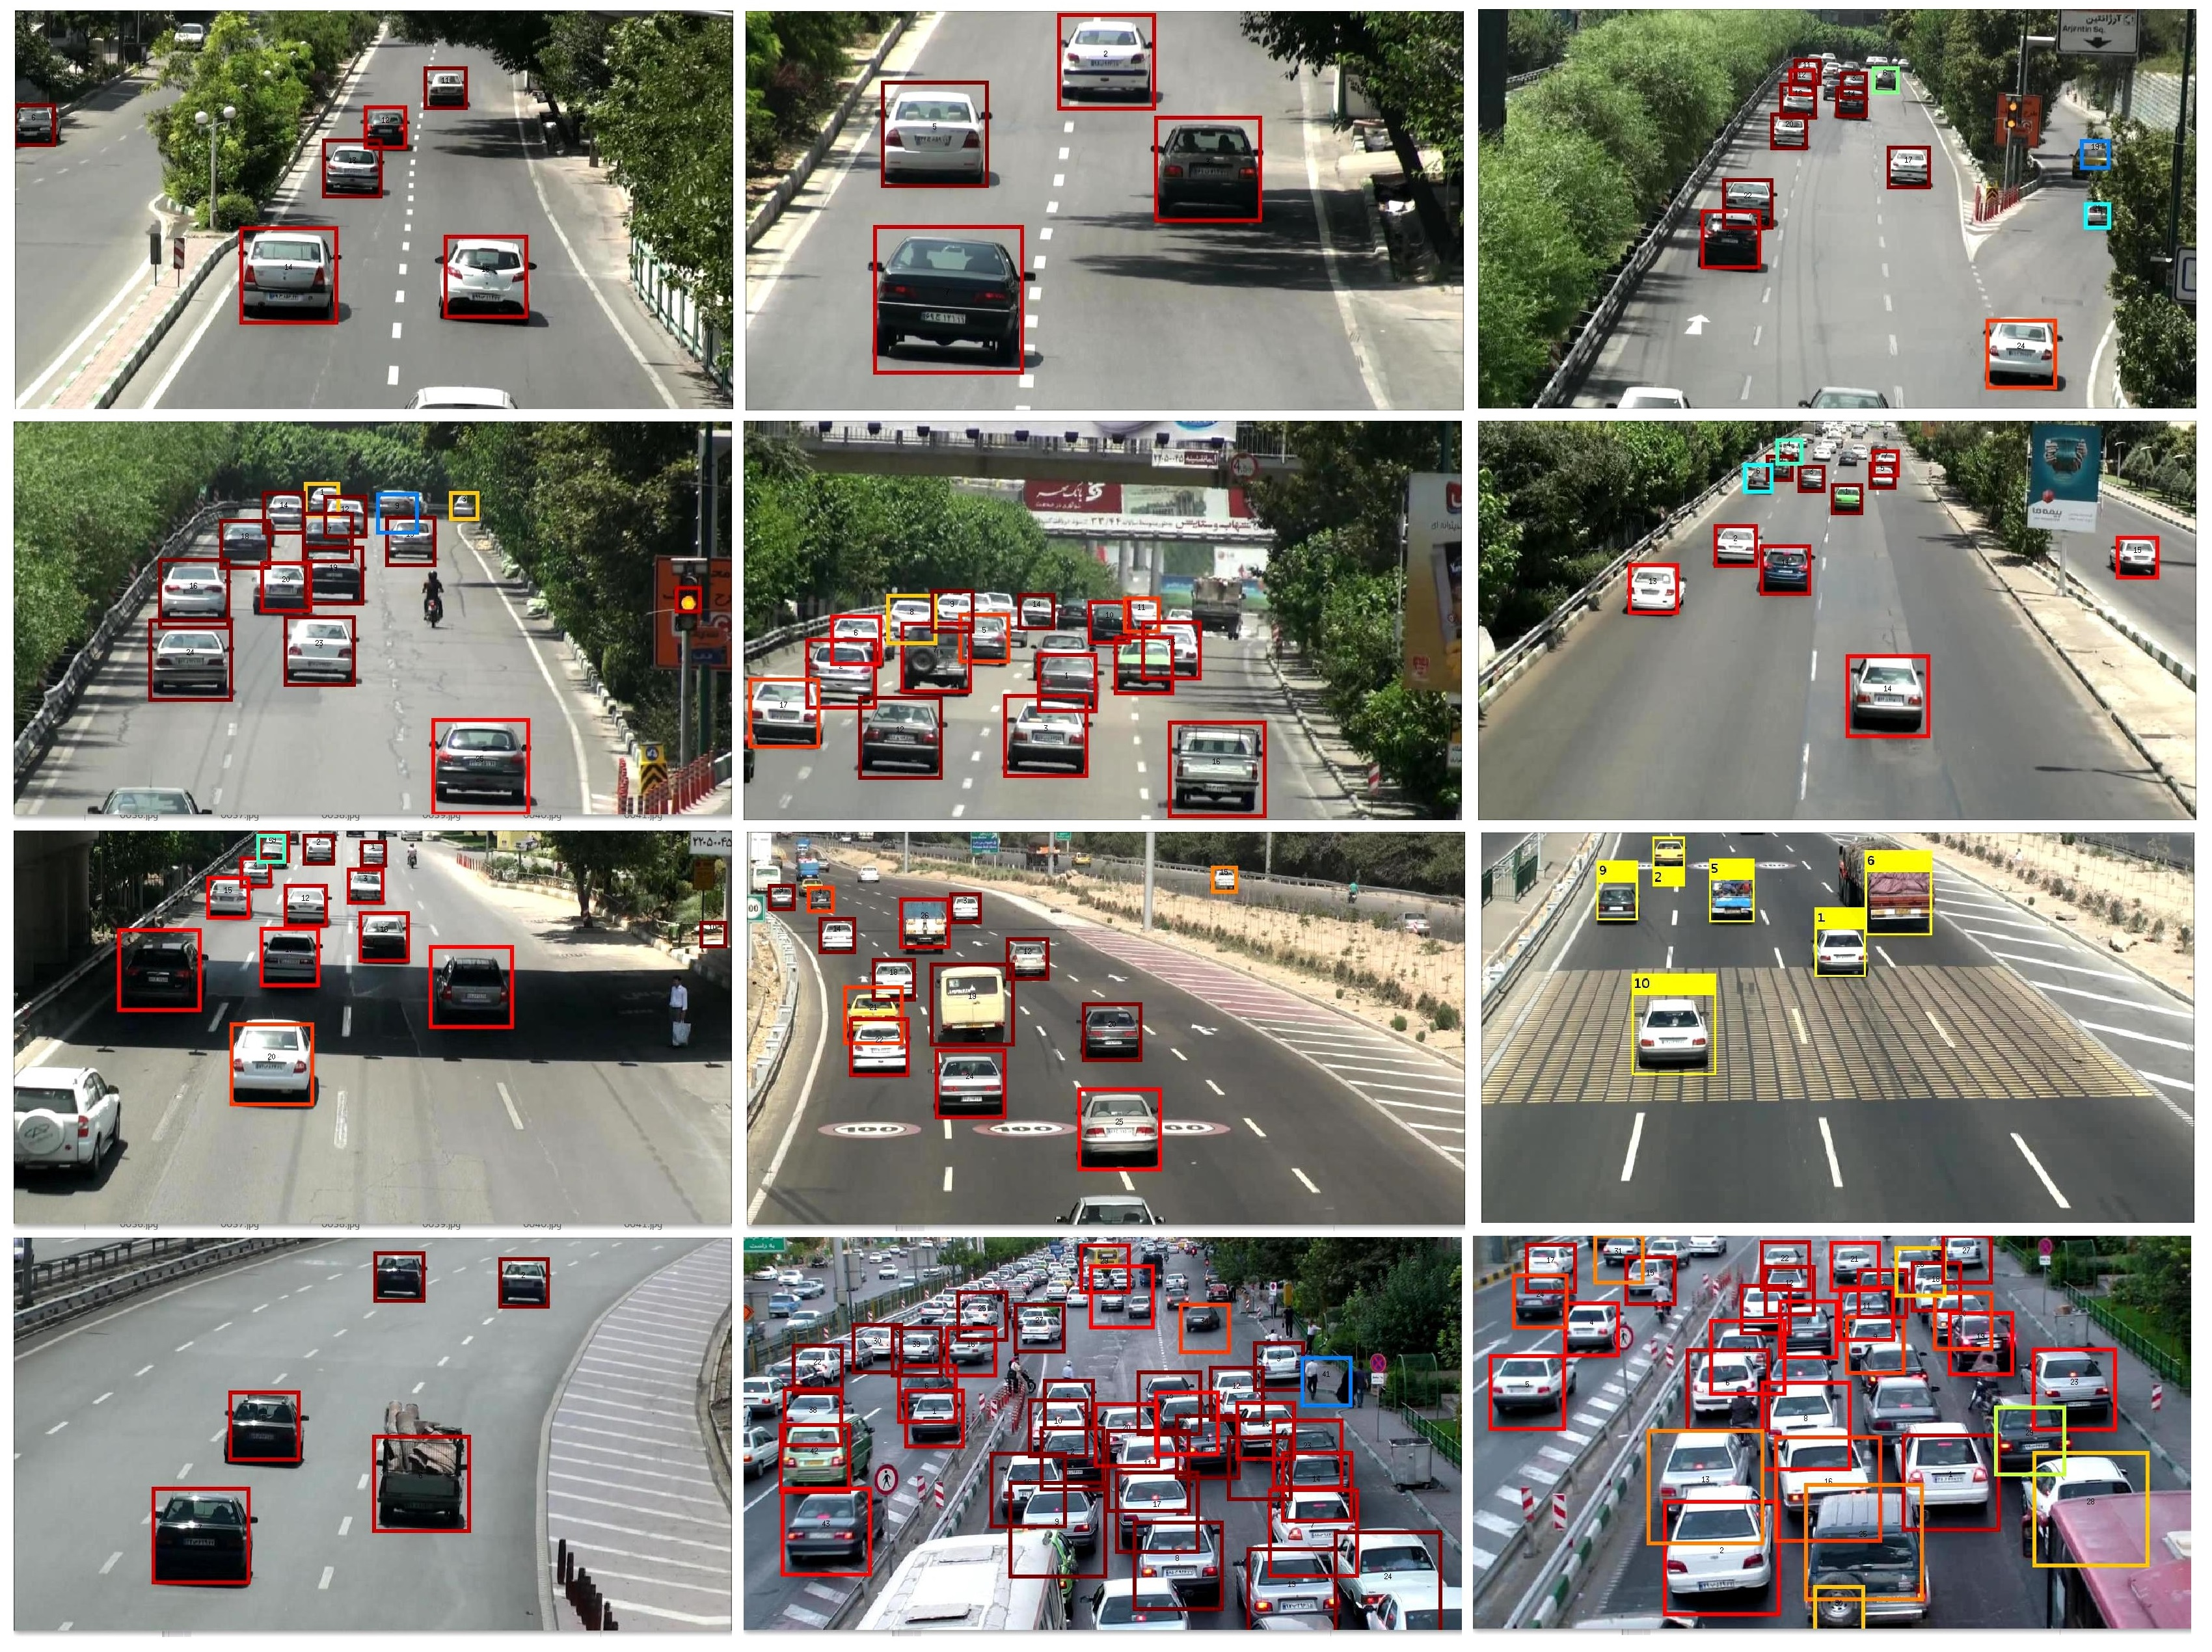
\includegraphics[width=\textwidth]{images/results.jpg}
	\caption{Result of our method in 12 videos of AUTCUP dataset}
	\label{results}
\end{figure*}


% conference papers do not normally have an appendix


% use section* for acknowledgement
\section*{Acknowledgment}


The authors would like to thank Mr. Agahi, member of technical committee of AUTCUP2015, for his helps.




\bibliography{ref}

\end{document}


